\documentclass[a4paper,12pt]{report}    %Article before

\usepackage{preamb}

\begin{document}

\lstset{style=output}
\thispagestyle{empty}
\centerline{\fontsize{60}{70}\selectfont\textbf{Embedded Real Time Systems}}
\vspace{10mm}
\vspace{40mm}
\centerline{\Huge\textbf{Assignment 2}}
\vspace{40mm}

\begin{table}[htb]
\fontsize{16}{30}\selectfont
\centering
\begin{tabular}{| p{85mm} | p{60 mm} |}
\hline
\textbf{Name:}                      &  \textbf{Students number:}     \\ \hline
Malthe Faurschou Tøttrup            &  201907882                     \\ \hline
Jakob Levisen Kvistgaard            &  201606374                     \\ \hline
\end{tabular}
\end{table}

\vspace{10mm}
\vspace{20mm}

\centerline{\large\textbf{\today}}
\centerline{\large\textbf{ }}


\tableofcontents
\pagestyle{ProjectReport}
\newpage
\lstlistoflistings
\newpage

\chapter{Assignment 2}
\section{Introduction}
\lstset{style=code}


The is the second assignment in Embedded Real Time Systems.
All source files can be found at: \url{https://github.com/levisen/ERTS}

\section{Exercise 3: Create a Console Application}
In this section we implement command 1) and 2) for the C-application. Command 1) reads the current value of the switches and writes this value to the LEDs. An example of using this command is shown if Fig. \ref{cmd1}, where the value of the switches is $9$ which is equal to $1001$ in binary. The this value can be interpreted as the switches being {['on', 'off', 'off' 'on']} respectively. As a result the LEDs will be also be {['on', 'off', 'off' 'on']} after executing the command. \\

\begin{figure}[h]
  \centering
  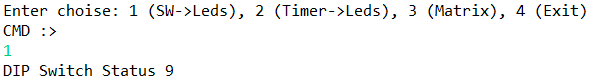
\includegraphics[scale = 1]{latex/figures/test1.PNG}
  \caption{Example output of command 1).}
  \label{cmd1}
\end{figure}

Command 2) increments the binary value of the LEDs every second in a loop using a counter variable as shown in Fig. \ref{cmd2}. The result is the LEDs counting up from $0-15$ in binary, resetting when the counter exceeds $15$. The loop can be exited by pressing one of the black buttons on the FPGA (not the red ones).

\begin{figure}[h]
  \centering
  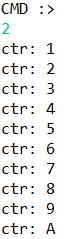
\includegraphics[scale = 1]{latex/figures/test2.PNG}
  \caption{Example output of command 2).}
  \label{cmd2}
\end{figure}

\section{Exercise 4: Create a Matrix Multiplication}
In this section we implemented command 3) which matrix multiplication of two predetermined matrices. The function implements formula $P = A \times B^T$ where it multiplies matrix A with the transpose of matrix B and writes the result to matrix P. For ease of implementation we instantiate matrix B as its transpose. The function has two different implementations where one is using the software and the other is using the hardware. The hardware implementation has been implemented using as \emph{matrix\_ip} ip\-core. The ip\-core has been imported into Vivado and instantiated and connected to the block\-design. The implementation of the two functions can be seen in Fig. \ref{matrix_mult}, in the implementation it is assumed that B is already ransposed (which it is). In the multiMatrixHard the specific registers have been located in from the matrix\_ip.h file. 

\begin{figure}[h]
  \centering
  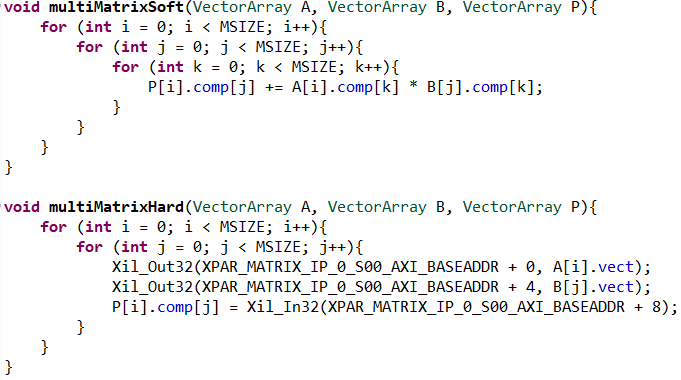
\includegraphics[scale = 1]{latex/figures/matrix_mult.PNG}
  \caption{Implementation of multiMatrixSoft and multiMatrixHard.}
  \label{matrix_mult}
\end{figure}
\newpage
\section{Exercise 5: Create a Hardware IP Acceleration}
In this section the two implemented matrix multiplication functions has been tested against each other to compare performance in terms of speed. The test is run then command 3) is executed. The output of issuing command 3) can be seen in Fig. \ref{cmd3}. The output prints first matrix A, then matrix B transposed, then the duration for executing multiMatrixSoft measured in clock cycles, then the resulting matrix P is printed. Afterwards the duration for executing multiMatrixHard is printed and the resulting matrix P, to ensure that the resulting matrix P is the same for both implementations. As we can see the software implementation is about twice (1767 clock cycles) as fast as the hardware (3880 clock cycles). It is expected that the software implementation would be faster than the hardware as the processor clock is 650 Mhz and the ip\-core clock has 100 Mhz. However, we would expect that the software would be about six times faster than the hardware. However, since the hardware is executing some instructions in parallel the software is only about twice as fast.

\begin{figure}[h]
  \centering
  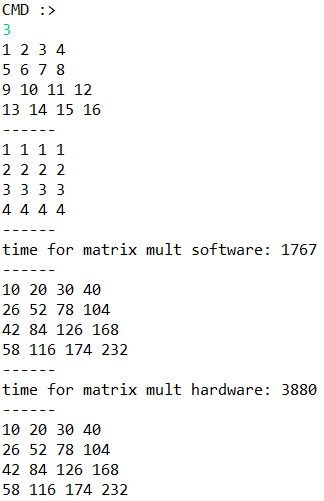
\includegraphics[scale = 1]{latex/figures/test3.PNG}
  \caption{Example output of command 3.}
  \label{cmd3}
\end{figure}

\section{Exercise 7: HLS exercise with SystemC}

In this exercise we will implement a hardware component controller for the switch buttons and LEDs on the Zybo board in SystemC. This component will then be synthesized using Vivado HLS to generate a Vidado IP Core, which will be then be used together with a software application.

\subsection{ADVIOS SystemC block}

From the header of the exercise we first implemented a pulse generator based on a 1 second counter. As we know the Hz rate, the thread implemented is just increasing the counter at every cycle and then resetting at time threshold. 

\lstinputlisting[language=C++, firstnumber=45, firstline=45, lastline=64, caption=Implementation of countThread()., label=27SOURCECOUNT]{code/src/assignment2/advios.cpp}

In iosThread we start reading the port signals at every cycle, if the control is equal to 0, and if the switch is not 8, we start the looping timer sequence. In case 0 < control < 15, we will bask the bit with switch input.

\lstinputlisting[language=C++, firstnumber=5, firstline=5, lastline=41, caption=Implementation of iosThread()., label=27SOURCEIOS]{code/src/assignment2/advios.cpp}

In figure \ref{FIG::27::GTKWAVE} it is shown what happens in the hardware loop, when the count reaches one cycle. In this example we increase the count at every 10 cycles, for testing and simulating purposes, but the result is the same. At 10 cycles the sec\_pulse signal is generated and wee sec an increment in both the sec\_counter and leds.

\begin{figure}[H]
  \centering
  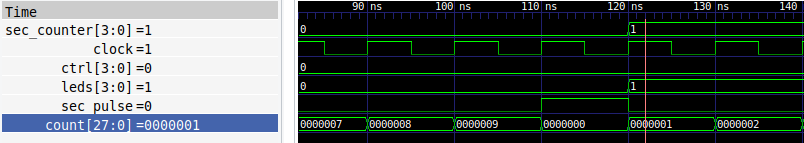
\includegraphics[width=\linewidth]{latex/figures/ass2_27_gtkwave.png}
  \caption{GTKWave output of simulation.}
  \label{FIG::27::GTKWAVE}
\end{figure}

\subsection{Utilizing Vivado HLS to generate IP core}

We used the guide from previous examples to generate the IP Core. Ultimately, this yielded the performance results in figure \ref{FIG::27::PERFORMANCE}. We can also see the allocation of Flip-Flops and Look-up tables in figure \ref{FIG::27::TRANSISTOR}.


\begin{figure}[H]
  \centering
  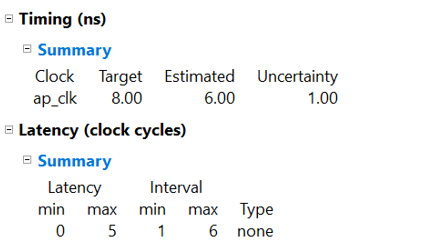
\includegraphics[scale=1]{latex/figures/ass2_27_performance.png}
  \caption{Performance of the IP-Core.}
  \label{FIG::27::PERFORMANCE}
\end{figure}
\begin{figure}[H]
  \centering
  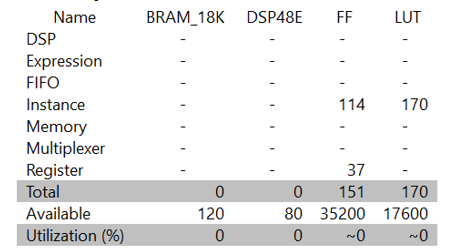
\includegraphics[scale=1]{latex/figures/ass2_27_hls_transistor_.png}
  \caption{Flip-flop and lookup table counts.}
  \label{FIG::27::TRANSISTOR}
\end{figure}

\subsection{Bitstream block generation in Vivado}

We then loaded the ip package from Vivado HLS into Vivado and added the components showed in the exercise. After adding some configurations and setting the outputs of the switch and LED's to external, the block diagram got validated. This is show in figure \ref{FIG::27::VIVADO}.

\begin{figure}[H]
  \centering
  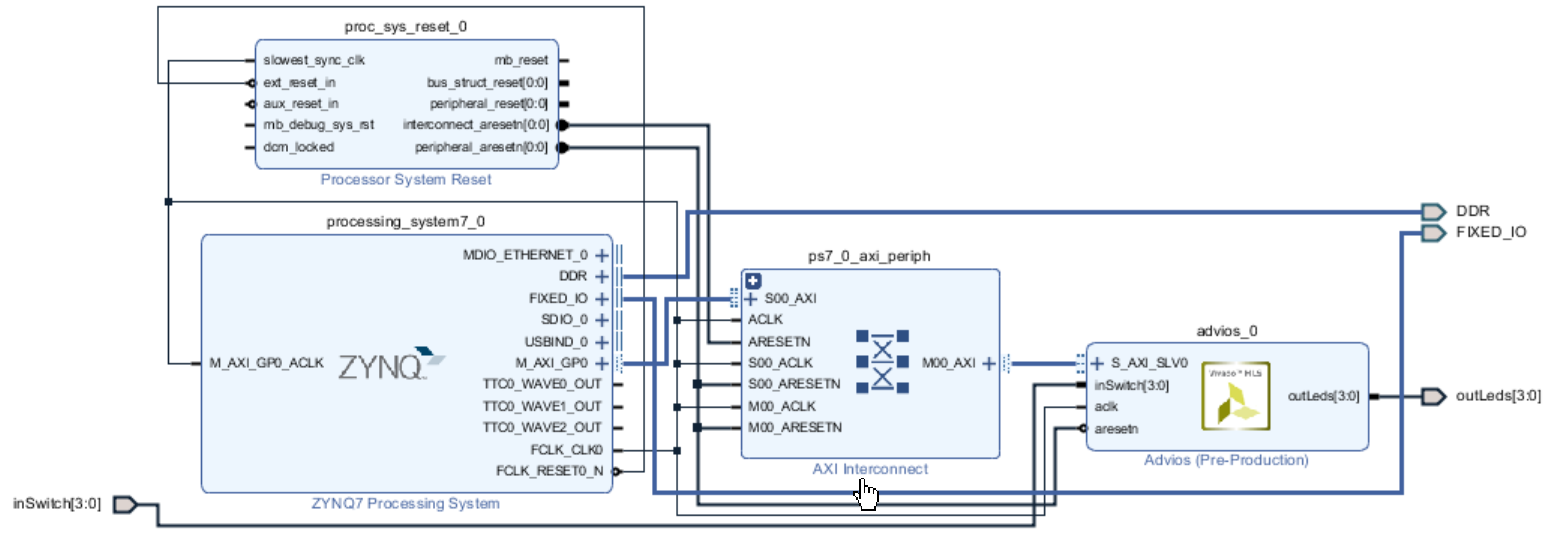
\includegraphics[width=\linewidth]{latex/figures/ass2_27_vivado_ip_design.png}
  \caption{Vivado IP block design.}
  \label{FIG::27::VIVADO}
\end{figure}

\subsection{Writing a test program using SDK}

The test program is using a object of type XAdvios to interact with the control signal on the Zybos unit. The test program is using a timer to change the control signal from 0 to 15, after 7 seconds. So that we can validate the bitwise and function and the 1 second pulse counter.
\begin{figure}[H]
  \centering
  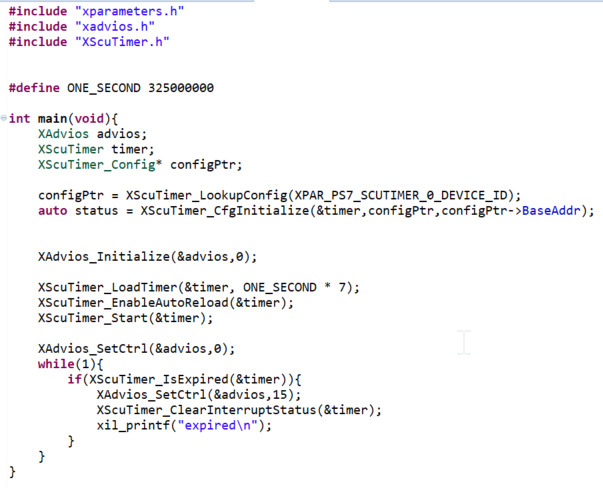
\includegraphics[width=\linewidth]{latex/figures/ass2_27_sdk_result.png}
  \caption{Testprogram in Xilinx SDK.}
  \label{FIG::27::XILINX}
\end{figure}


\subsection{Results}

The counter works, you just got to believe in us. While running the Zybo unit in counting mode uwe use a control signal of 0. We can then disable the counter and turn of the LED's by setting the switch signal to 8 (1000 in binary). This is shown in figure \ref{FIG::27::MODE0}. The same switch input will not turn off the LED's when running with another control input (0 < control < 15), shown in figure \ref{FIG::27::MODE1}

\begin{figure}[H]
  \centering
  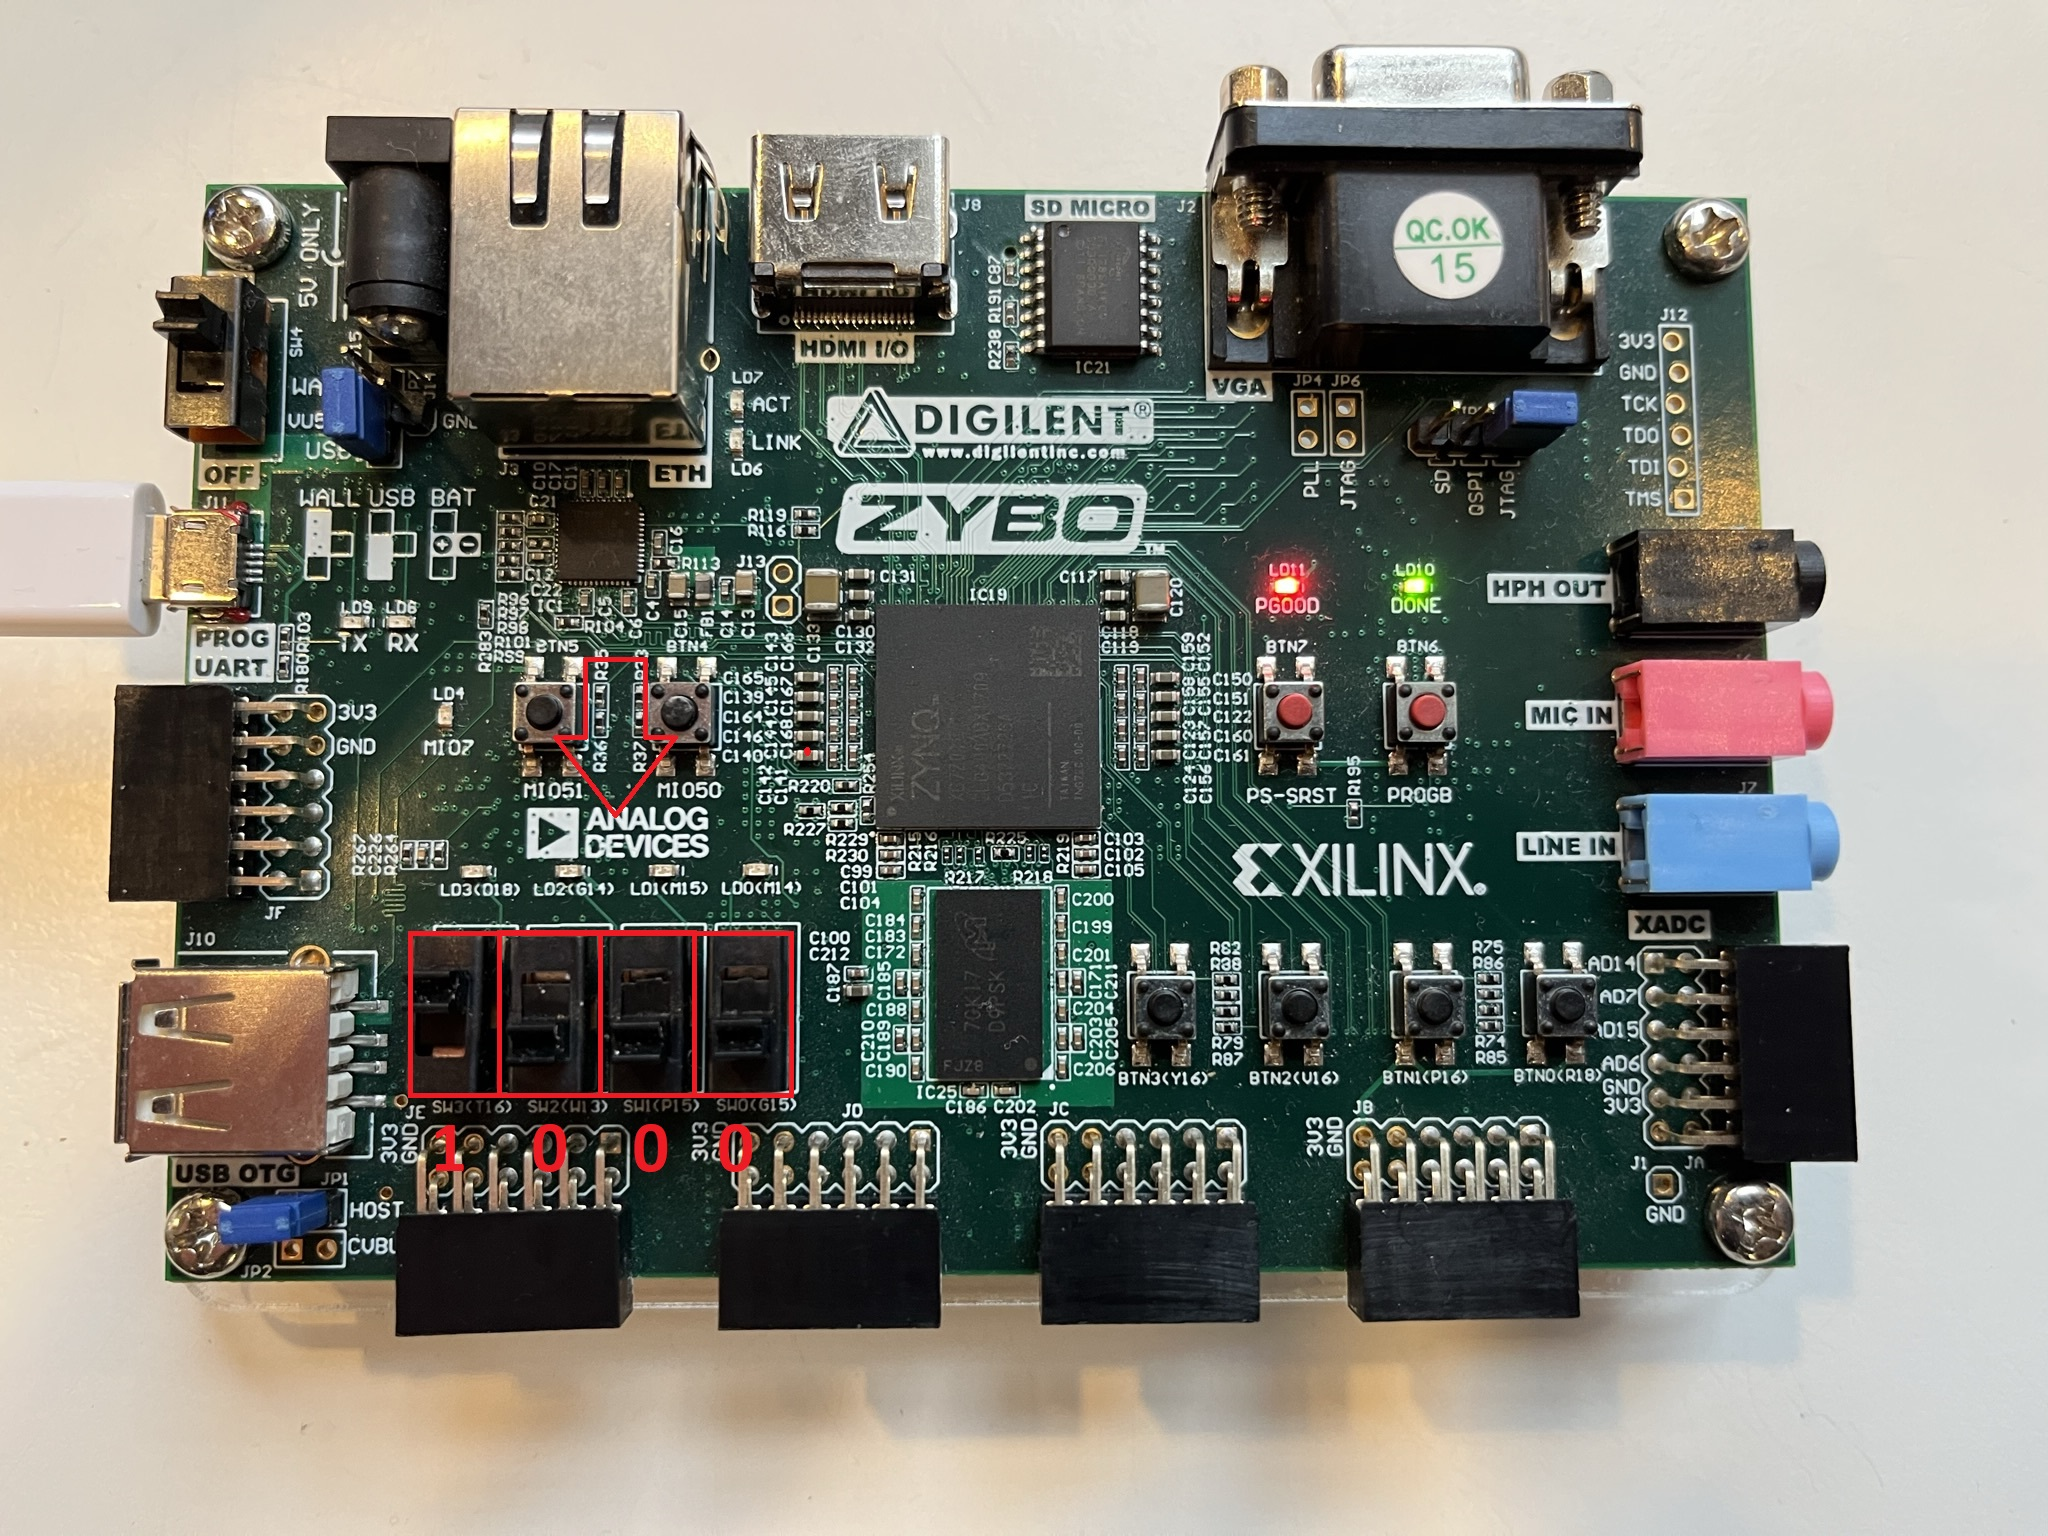
\includegraphics[width=\linewidth]{latex/figures/ass2_27_result_0x8.jpeg}
  \caption{Test result of running the node in control mode 0, with switch input 8}
  \label{FIG::27::MODE0}
\end{figure}

\begin{figure}[H]
  \centering
  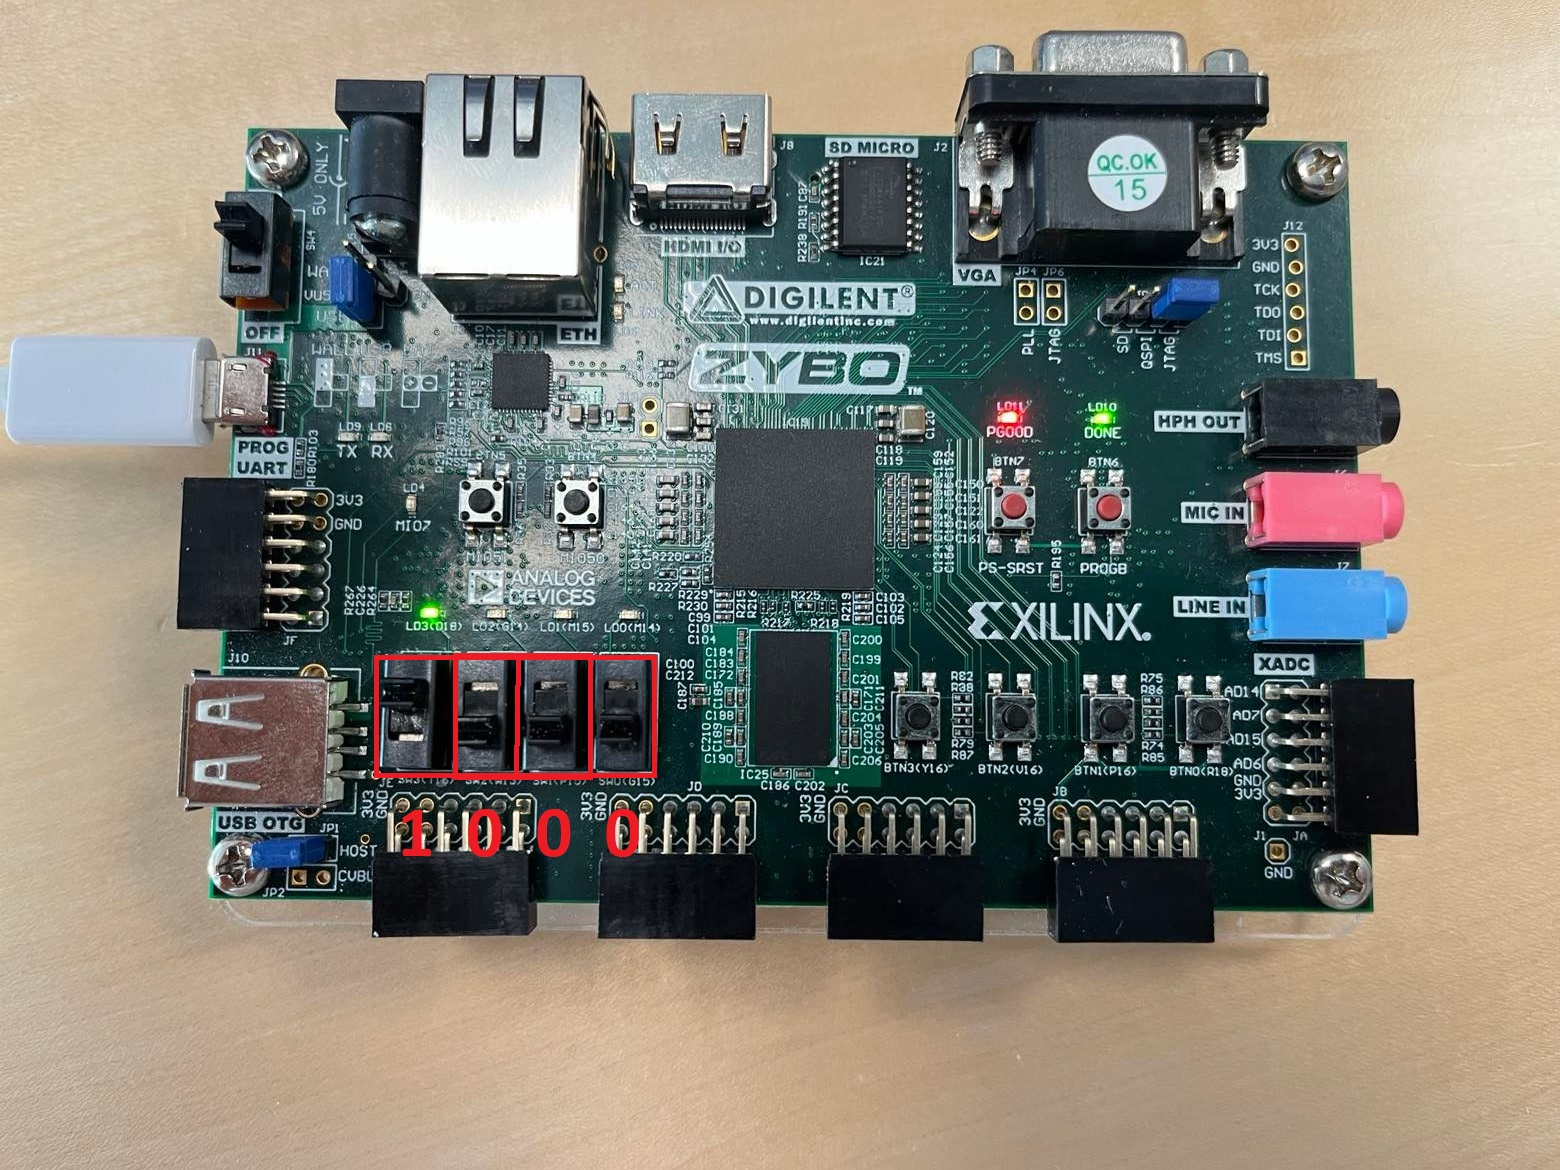
\includegraphics[width=\linewidth]{latex/figures/ass2_27_crl15_result.jpg}
  \caption{Test result of running the node in control mode 9 with switch input 8.}
  \label{FIG::27::MODE1}
\end{figure}

In figure \ref{FIG::27::MODE2} and \ref{FIG::27::MODE3} we see the difference when using the bitwise and function that is implemented. We are using a control signal input of 9 which is 1001 in binary. In figure \ref{FIG::27::MODE2} we see that all the LEDs are turned on, likewise the bits (1001). In the \ref{FIG::27::MODE3}, we see that the same LED's are flashing, even though the switch is 15 (1111).

\begin{figure}[H]
  \centering
  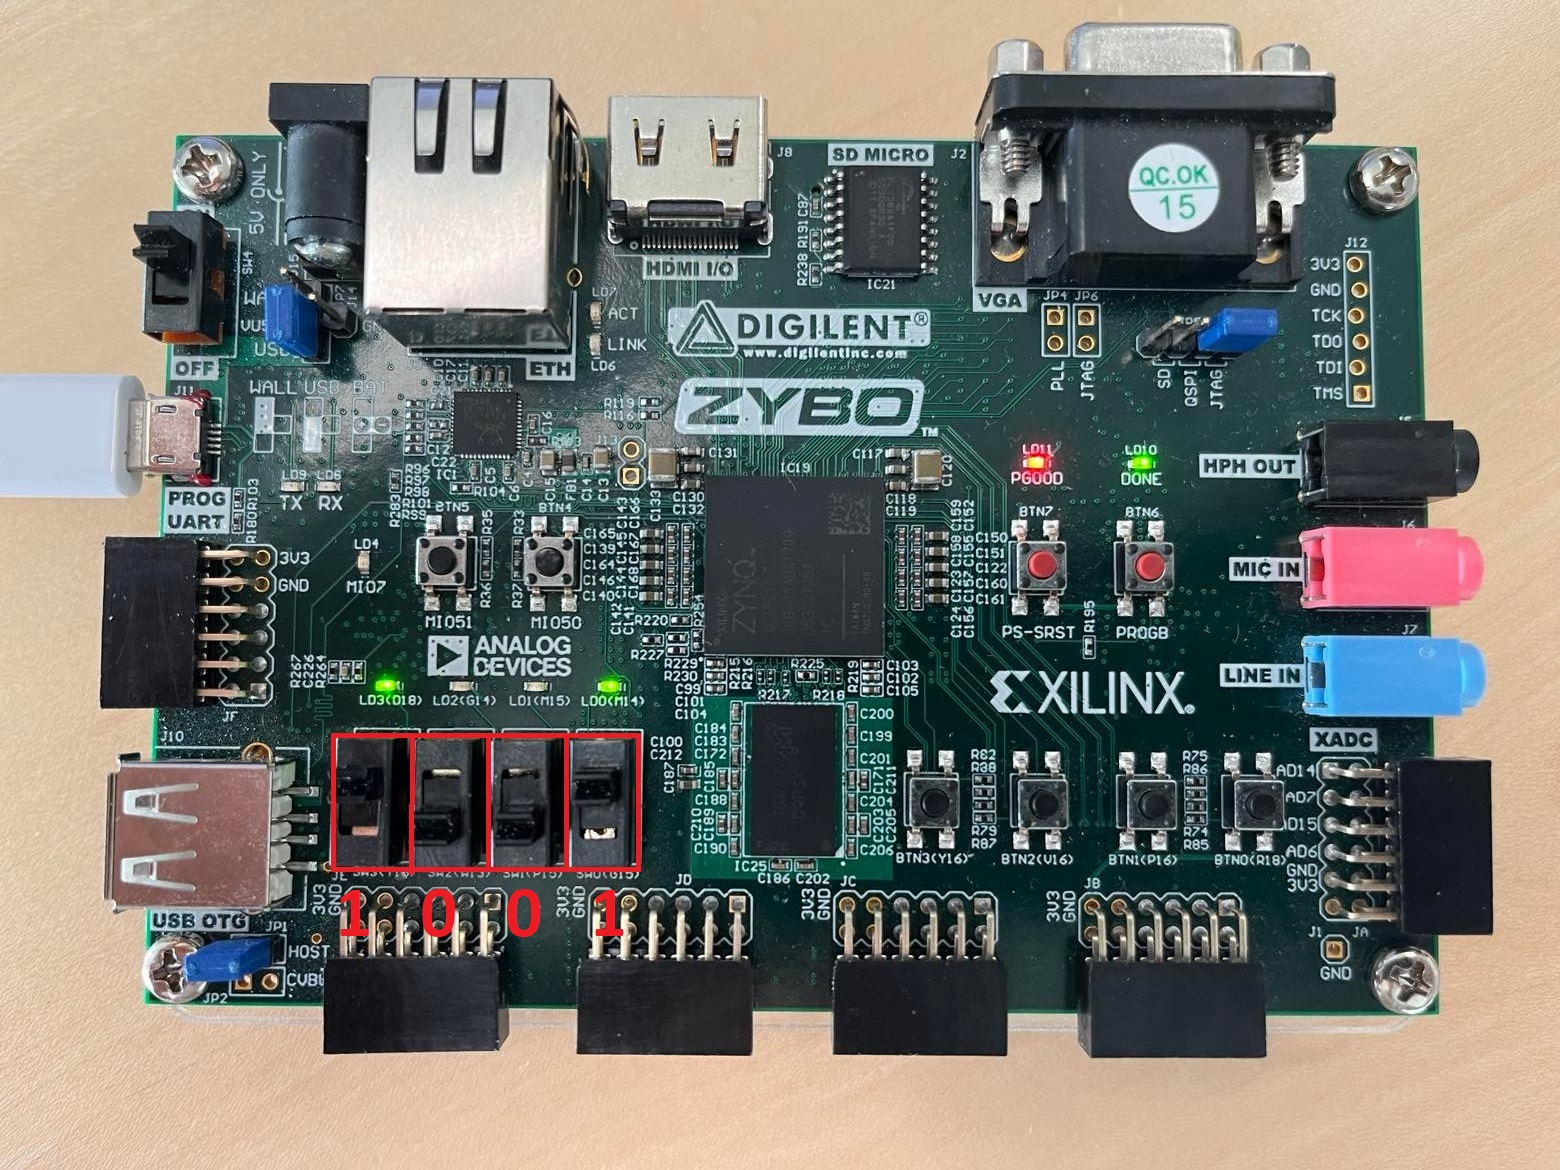
\includegraphics[width=\linewidth]{latex/figures/ass2_27_1001_0.jpg}
  \caption{Test result of running the node in control mode 9 with switch input 9.}
  \label{FIG::27::MODE2}
\end{figure}

\begin{figure}[H]
  \centering
  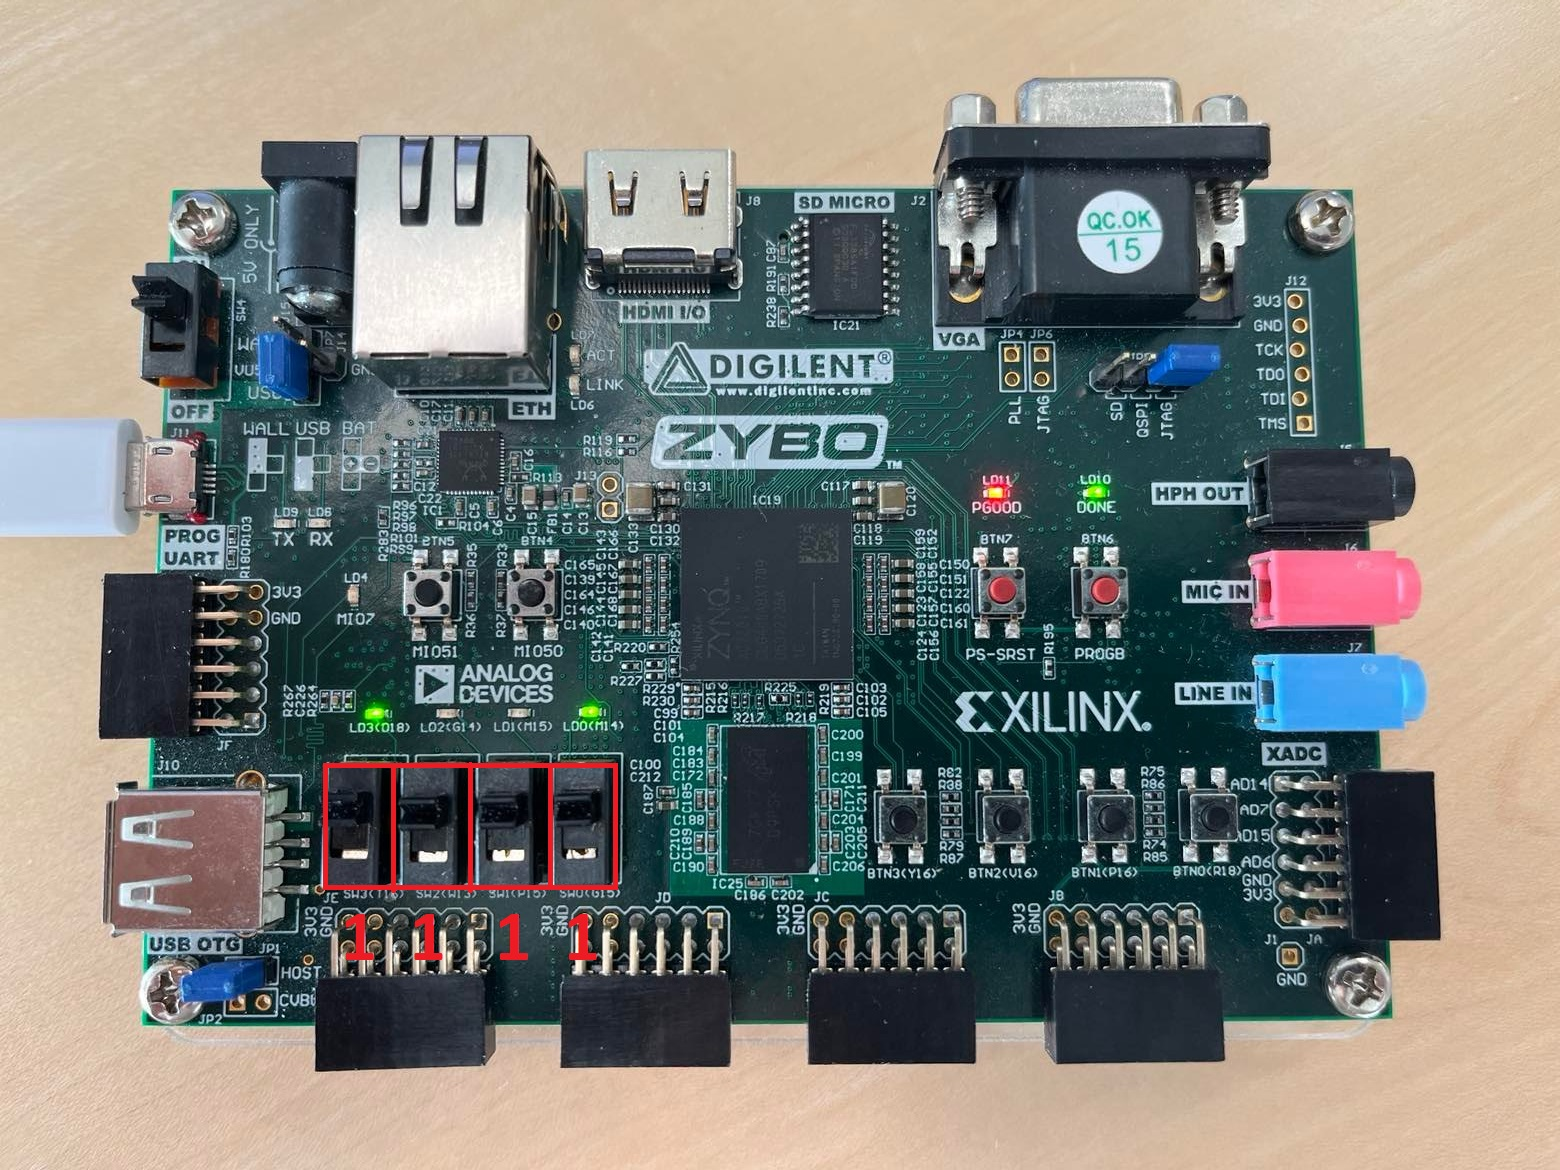
\includegraphics[width=\linewidth]{latex/figures/ass2_27_1001_1.jpg}
  \caption{Test result of running the node in control mode 9 with switch input 15.}
  \label{FIG::27::MODE3}
\end{figure}

\end{document}
